\documentclass[doc, 12pt, a4paper,floatsintext]{apa7} 
\setcounter{secnumdepth}{3}
% Packages
\usepackage{tikz}
\usetikzlibrary{arrows.meta, positioning}
%\usepackage[utf8]{inputenc}
\usepackage{epigraph}
\usepackage[T1]{fontenc}
\usepackage{lmodern}
\usepackage{hyperref}
\usepackage{xurl}
\usepackage{graphicx}
\usepackage{array}
\usepackage{ragged2e}
\usepackage{adjustbox}
\usepackage{booktabs}
\usepackage{caption}
\usepackage{microtype}
\usepackage{setspace}
\usepackage{amsmath}
\usepackage{anyfontsize}
\newcolumntype{L}[1]{>{\RaggedRight\arraybackslash}p{#1}}
\justifying
% Configure APA7 Citations
\usepackage[style=apa, backend=biber]{biblatex}
% in console
% file.remove("gatopardo.aux", "gatopardo.bcf", "gatopardo.bbl", "gatopardo.blg", "gatopardo.run.xml")
% system("pdflatex gatopardo.tex")
% system("biber gatopardo")
\addbibresource{Premieres.bib} 

% ============================================================
% APA 7 Metadata Structure (All required elements)
% ============================================================
\title{The Instability Itself Is the Institution: Ministerial 
Survival and Institutional Learning in Peru, 1821--2026}
\shorttitle{The Instability Itself Is the Institution}

\author{Jose Manuel Magallanes Reyes}
\leftheader{Magallanes Reyes}
\authorsaffiliations{Departamento de Ciencias Sociales e 
Instituto PULSO, Pontificia Universidad Cat\'olica del Per\'u}
% This satisfies the abstract requirement. If you don't want to write it yet, 
% just leave the text inside empty, but keep the command!
\abstract{Why do political systems that change so much change so 
little in how they govern? This paper addresses that question 
through an original dataset of 1,062 ministerial spells covering 
five portfolios in Peru from 1821 to 2026. Rather than treating 
ministerial duration as the outcome to be explained, we treat it 
as a signal: an observable trace of the continuity conditions 
under which governing experience either accumulates into 
institutional knowledge or is repeatedly lost. We organize the 
analysis around two analytical heuristics. The first is the 
institutional epoch --- the path-dependent period between 
critical junctures --- which captures whether successive 
historical ruptures produced durable improvements in continuity 
conditions. The second is the protective belt --- a localized 
architecture of external accountability relationships that, where 
it exists, insulates certain ministries from the political logic 
governing the rest of the cabinet. Kaplan--Meier survival curves, 
log-rank tests, and Cox proportional hazards models show that 
epochs explain ministerial survival far better than individual 
traits or portfolio membership, and that continuity conditions 
did not improve monotonically across two centuries. The largest 
shift in the data occurred between the Oligarchic State and the 
Power-Sharing epoch; the most recent democratic period represents 
a partial regression toward the founding pattern of chronic 
interruption. The protective belt emerges only after 1993, when 
external accountability structures raised the cost of Economy 
minister replacement beyond what domestic political pressure 
alone could sustain. The central theoretical finding is that 
chronic ministerial instability in Peru is not evidence of absent 
institutions but of a durable informal one: the escape valve 
through which political pressure is absorbed without producing 
structural change. The instability itself is the institution.}

\usepackage{Sweave}
\begin{document}
\Sconcordance{concordance:gatopardo.tex:gatopardo.Rnw:1 48 1 1 0 2 1 1 4 525 1 1 6 8 %
1 1 85 31 0 1 2 104 1 1 102 1 2 37 1 1 91 22 0 1 3 28 1 1 65 1 2 19 1 1 %
148 1 3 13 1 1 122 1 2 77 1}



\maketitle 
\tableofcontents

\epigraph{``Se vogliamo che tutto rimanga com'è, bisogna che tutto cambi.''}
{\textit{Il Gattopardo} \\ Giuseppe Tomasi di Lampedusa, 1958}


% ============================================================
\section*{Introduction}
% ============================================================


Governing is hard. Education, health, public safety, and economic development are not technical problems with known solutions, but complex social challenges that demand sustained institutional effort. Good policy takes time to design, time to implement, and even longer to produce visible social outcomes. Good practices diffuse gradually. Organizations accumulate knowledge slowly. Institutional learning emerges only when that accumulated knowledge is preserved, transmitted, and refined across successive administrations. Citizens experience meaningful change only after years of coherent action in the same direction. In the long run, successful governance depends less on isolated political decisions than on the organizational conditions that allow knowledge to persist beyond individual officeholders.

After more than two hundred years of republican life, the Peruvian political class has repeatedly changed governments, cabinets, constitutions, and political coalitions. Yet the underlying pattern remains remarkably stable. Each new administration appoints a cabinet whose members understand, implicitly or explicitly, the terms of their engagement: they are expected to manage complexity on behalf of the president, but they may also be sacrificed whenever political pressure demands a visible response. Their departure rarely resolves the conflict that triggered it. The resignation of a premier or any other minister may relieve immediate pressure, but it seldom addresses the underlying causes of crisis. Cabinet reshuffles therefore signal political responsiveness without necessarily producing institutional correction.

This persistence should not be mistaken for an absence of adaptation. Political actors continuously learn how to navigate constitutional ambiguities, manage public blame, and deploy ministerial replacement as a mechanism for absorbing political pressure. If the political class has accumulated any expertise, it has largely been in reproducing established responses to crisis rather than transforming the institutional conditions that generate those crises. Governments change. Ministers change. Yet the repertoire through which instability is managed remains remarkably stable. This cycle has characterized much of Peru's republican history.

Political scientists often describe this type of persistence through the concept of path dependence, whereby accumulated institutional choices progressively constrain subsequent alternatives. Yet paths do break. Roman \textcite{krznaric_how_2024} argues that transformative institutional change requires what he calls a \emph{disruption nexus}: a major crisis, social movements capable of amplifying that crisis, and a compelling institutional idea ready to occupy the political space created by disruption. France's Fifth Republic illustrates this dynamic. The Algerian War provided the crisis, Gaullism supplied the political movement, and constitutional redesign centered on a strong executive offered the institutional solution. The resulting transformation was not the product of a single event but the culmination of decades of unresolved executive instability. More importantly, it fundamentally altered the conditions under which political continuity was produced. The legacy of the Fifth Republic was therefore not merely institutional reform, but a durable change in the patterns of executive stability that had characterized French politics for more than a century.

Prior to the Fifth Republic, France exhibited levels of executive instability comparable to those observed throughout much of Peru's republican history. Figure~\ref{fig:premiers} illustrates this similarity. Peru reached twenty-three premier appointments during the 1890s, while France reached twenty during the 1930s. After 1958, however, the trajectories diverged sharply. French premier appointments declined to a stable range of three to six per decade and have remained there ever since, whereas Peru has gradually returned to levels characteristic of the nineteenth century. Peru has experienced no shortage of potential disruption nexuses---or, as they will later be conceptualized in this paper, critical junctures: independence without effective state-building, the War of the Pacific, hyperinflation, political violence, the collapse of the Fujimori regime, and the prolonged constitutional crisis beginning in 2016. Each represented a historical moment in which alternative institutional trajectories became plausible.

The central question, however, is not whether institutional change occurred. Peru's republican history is full of constitutional reforms, regime transitions, and political ruptures. The more fundamental question is whether these transformations altered the organizational conditions under which knowledge could be preserved, accumulated, and transmitted over time. From this perspective, a critical juncture matters not simply because it generates new institutional arrangements, but because it may establish a durable political framework capable of reshaping the conditions under which organizations accumulate knowledge and governments learn. France appears to have experienced such a transformation after 1958. Peru's trajectory raises the possibility that institutional innovation and organizational learning do not necessarily coincide.

\begin{figure}[!htbp]
    \centering
    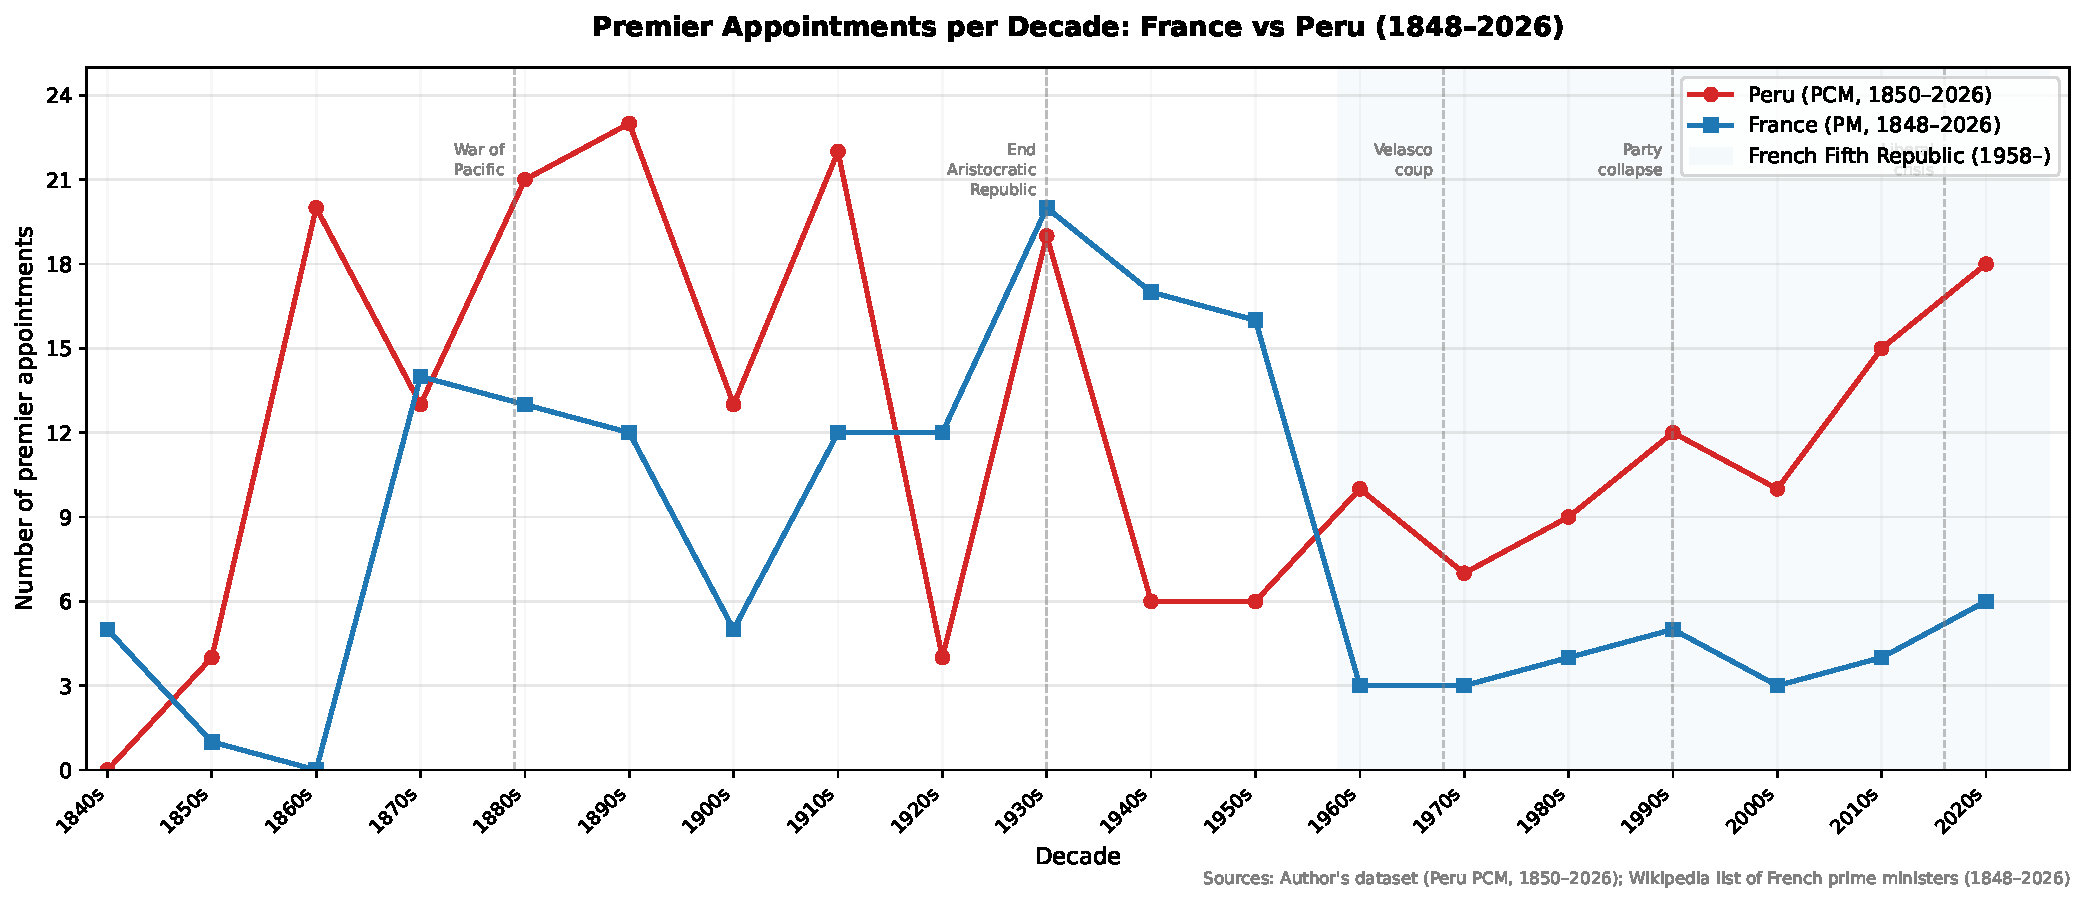
\includegraphics[width=\textwidth]{premiers_decennial.pdf}
    \caption{Premier Appointments per Decade: France vs.\ Peru, 1848--2026.\\
    \textit{Sources}: Author's dataset (based on \textcite{galvez_montero_historia_2016, galvez_montero_historia_2016-1}); Wikipedia list of French prime ministers (1848--2026).}
    \label{fig:premiers}
\end{figure}

This paper approaches that question through ministerial continuity. Ministerial duration is not interpreted as evidence of organizational learning itself. Rather, it constitutes observable evidence about the organizational conditions under which knowledge may accumulate. Organizations do not preserve knowledge because particular individuals remain indefinitely in office. Instead, sustained continuity creates opportunities for organizational routines, institutional memory, policy procedures, and accumulated expertise to be retained and transmitted despite inevitable personnel turnover. Ministerial continuity therefore represents a necessary---although not sufficient---condition for organizational knowledge accumulation.

Political science has traditionally examined these issues through separate research traditions. Ministerial duration has been analyzed using survival and event-history methods, whereas long-term institutional development has largely been studied through the comparative-historical literature on path dependence and critical junctures. This paper connects these traditions by reconceptualizing ministerial continuity as an observable indicator of the organizational conditions required for knowledge accumulation and institutional learning.

The empirical strategy follows two complementary heuristics derived from the theoretical framework developed below. The first examines variation in ministerial continuity across historically distinct political frameworks in order to evaluate how opportunities for organizational knowledge accumulation changed over time. The second compares continuity across ministerial portfolios operating within the same political framework, recognizing that some organizations may become partially insulated from the broader political dynamics affecting the cabinet as a whole. Together, these perspectives distinguish historical variation from organizational variation in the conditions under which organizational knowledge may accumulate.

The question guiding this study is straightforward: \emph{Have Peru's successive political frameworks generated different opportunities for the accumulation of organizational knowledge?}

This question cannot be answered directly because organizational knowledge is not directly observable in historical records. Instead, the analysis evaluates the necessary organizational condition under which knowledge may accumulate: continuity. If organizational continuity constitutes a prerequisite for knowledge accumulation, then systematic differences in ministerial continuity should reveal systematic differences in the opportunities available for organizations to preserve, accumulate, and transmit knowledge over time.

The theoretical framework translates this general question into three empirical questions. \emph{First}, what continuity conditions characterized Peru's successive political frameworks? \emph{Second}, did those continuity conditions differ systematically across political frameworks? \emph{Third}, within the same political framework, did some ministerial portfolios systematically exhibit greater continuity than others?

To answer these questions, we construct an original dataset of individual ministerial spells covering the period from 1821 to 2026. The analysis focuses on five portfolios that capture distinct organizational functions within the executive branch. The Presidency of the Council of Ministers (PCM) represents the political center responsible for coordinating cabinet action and maintaining executive cohesion. The Ministry of Economy and Finance (MEF) represents the technocratic center responsible for fiscal and macroeconomic policy. The Ministries of Interior, Health, and Education represent policy sectors confronting some of Peru's most persistent governance challenges according to official yearly surveys \parencite{inei_encuesta_2024}. Ministerial spells are subsequently organized into historically distinct political frameworks derived from Peru's critical junctures \parencite{lopez_jimenez_peru_2025}. Combining descriptive analyses with survival models, the study evaluates how organizational continuity varied across political frameworks and ministerial portfolios, thereby providing empirical evidence about the organizational conditions under which knowledge accumulation becomes possible.


%%%

% ============================================================
\section{Literature Review}
% ============================================================

The political science literature on ministerial survival has converged around two broad families of explanations. The first explains variation in ministerial tenure through characteristics of ministers themselves. The second emphasizes the political and institutional environments within which ministers operate. Table~\ref{tab:lit_review} summarizes the principal covariates identified across the core studies.

\begin{table}[!htbp]
\centering
\caption{Trait-based and Context-based Predictors of Ministerial Survival}
\label{tab:lit_review}
\scriptsize
\hbadness=10000
\setlength{\tabcolsep}{3pt}
\renewcommand{\arraystretch}{0.78}
\begin{adjustbox}{max width=\textwidth,max totalheight=.82\textheight}
\begin{tabular}{L{.27\textwidth}L{.34\textwidth}L{.34\textwidth}}
\toprule
\textbf{Author(s)} & \textbf{Trait-based} & \textbf{Context-based} \\
\midrule
\textcite{blondel_ministerial_1988} & Career duration; parliamentary vs.\ managerial profile & Party system norms; head-of-government style; country context \\
\midrule
\textcite{huber_replacing_2008} & Ideological distance from government center; PM party membership; portfolio importance & Coalition type; minority government; electoral volatility; party fractionalization \\
\midrule
\textcite{dewan_corrective_2005} & Resignation issue salience; ministerial seniority & PM support level; media attention; single-party vs.\ coalition system \\
\midrule
\textcite{fischer_duration_2012} & Age; education; gender; portfolio rank & PM popularity; regime type; frequency of resignation calls \\
\midrule
\textcite{camerlo_minister_2015} & Portfolio type; technocrat/partisan/outsider profile; first cabinet appointment & Protests; scandals; electoral calendar; term limits; reelection rules \\
\midrule
\textcite{camerlo_government_2024} & Partisan rank within party hierarchy (leader, high-rank, low-rank, newcomer, shadow, defector) & Party government model applicability; regime type; party institutionalization level \\
\midrule
\textcite{feliu_ribeiro_foreign_2023} & Technical expertise; presidential group membership; prior electoral experience (\emph{risk factor}) & Economic growth; GDP per capita; legislative powers; regime type; portfolio area \\
\midrule
\textcite{mejia_es_2021} & Education; gender; regional origin; prior elected office & Coalition type; legislative majority; party-system change \\
\midrule
\textcite{alexiadou_commitment_2019} & Technocratic profile; non-partisan status; reform commitment & Economic crisis severity; electoral system type; party control of portfolio \\
\midrule
\textcite{baturo_office_2014} & Personal traits as time-invariant officeholder effects (education, prior career) & Regime institutionalization; personalization vs.\ office-based authority \\
\midrule
\textcite{jara_iniguez_rotacion_2019} & Managerial performance lifecycle (inverted-U over tenure) & Presidential appointment and dismissal capacity; political trust as selection criterion \\
\bottomrule
\end{tabular}
\end{adjustbox}
\end{table}

% ============================================================

\subsection{Trait-Based Explanations of Ministerial Survival}

Trait-based approaches explain ministerial survival through characteristics of the officeholder. Across different institutional settings, scholars have shown that ministers' professional backgrounds, political careers, partisan affiliations, and personal resources influence their probability of remaining in office. Early studies emphasized broad distinctions between managerial and parliamentary profiles, as well as the effects of career trajectories and prior political experience \parencite{blondel_ministerial_1988}. Subsequent work expanded the range of relevant characteristics to include age, education, gender, portfolio rank, and seniority within government \parencite{fischer_duration_2012,dewan_corrective_2005}.

More recent research has refined these categories by focusing on the organizational and political resources that ministers bring to office. Feliú Ribeiro and López Burian show that technical expertise and membership in presidential networks increase ministerial survival, while prior electoral experience may paradoxically operate as a risk factor \parencite{feliu_ribeiro_foreign_2023}. Across four Latin American countries between 1945 and 2020, career politicians proved more vulnerable to dismissal than technocrats. The finding suggests that ministerial value cannot be reduced to political experience alone; survival depends on the type of resources political leaders seek to preserve.

The literature has also moved beyond simple dichotomies between partisan and non-partisan ministers. Camerlo and Castaldo argue that partisan affiliation conceals substantial variation in the strength of a minister's relationship with the party organization. Their framework distinguishes among leaders, high-ranks, low-ranks, newcomers, shadows, and defectors according to levels of engagement, consolidation, and hierarchical position within the party \parencite{camerlo_government_2024}. Applied to the Argentine cabinet under Alberto Fernández, this approach reveals that apparently strong partisan cabinets may actually consist of ministers with limited organizational leverage over their parties \parencite{camerlo_poderes_2024}. Ministers sharing the same partisan label therefore possess very different capacities to withstand political pressure.

Taken together, these studies demonstrate that ministerial duration is shaped by who ministers are. Technical expertise, organizational embeddedness, political experience, and personal resources all influence survival prospects. Yet the effects of these traits depend fundamentally on the environments in which ministers operate. The same characteristic may be rewarded in one institutional setting and penalized in another. This observation leads naturally to the second major family of explanations.

% ============================================================

\subsection{Context-Based Explanations of Ministerial Survival}

Context-based approaches explain ministerial survival through characteristics of the political environment rather than characteristics of individual ministers. Ministers survive or fail because of the institutional and political constraints surrounding them.

The comparative literature consistently identifies coalition dynamics as a central determinant of ministerial duration. Coalition type, minority government status, electoral volatility, and party-system fragmentation all shape the likelihood of ministerial replacement independently of individual characteristics \parencite{huber_replacing_2008}. Similarly, political crises, scandals, protests, electoral calendars, and term limits alter the incentives presidents face when deciding whether to retain or dismiss ministers \parencite{camerlo_minister_2015,alexiadou_commitment_2019}. Even macroeconomic performance influences survival probabilities by modifying the broader political environment within which governments operate \parencite{feliu_ribeiro_foreign_2023}.

The case literature illustrates these mechanisms particularly clearly. For Colombia, Mejía Guinand et al.\ find that although individual characteristics matter, the institutional configuration of the political system ultimately determines the range within which those characteristics can operate \parencite{mejia_es_2021}. Constitutional reforms, changes in party-system structure, and coalition arrangements alter the political logic governing ministerial careers. Similar conclusions emerge from Chile, where Avendaño and Dávila show that ministerial turnover during the Concertación governments was driven primarily by coalition management rather than by individual performance. Finance ministers consistently exhibited the longest tenures regardless of their personal characteristics \parencite{avendano_rotacion_2012}.

Recent work has also refined the contextual analysis of ministerial portfolios. Portfolio importance has traditionally been measured through expert rankings that assign ministries a single level of salience. Camerlo and Martínez-Gallardo argue that such measures obscure important differences among ministries, particularly in contexts characterized by weak party institutionalization \parencite{camerlo_por_2022}. Their framework decomposes ministerial value into policy-management capacity, discretionary resource allocation, political agenda influence, and inter-portfolio coordination authority. Different political environments activate different dimensions of portfolio value, producing distinct survival incentives for presidents and ministers alike.

Taken together, these studies demonstrate that ministerial survival depends not only on who ministers are but also on where they operate. Institutional structures, coalition arrangements, political crises, economic conditions, and portfolio characteristics jointly define the opportunities and constraints governing ministerial careers.

% ============================================================

\subsection{Reinterpreting Ministerial Continuity}

The two families of explanations are not competing research programs. Virtually every empirical study combines individual and contextual covariates, with political environments conditioning the effects of ministerial characteristics. Together, these studies provide a rich understanding of why some ministers survive longer than others.

Despite their differences, however, they share an implicit assumption: ministerial duration is itself the phenomenon to be explained. Consequently, continuity is interpreted primarily as the outcome of cabinet management, coalition bargaining, institutional constraints, or individual characteristics. This common orientation leaves unexplored a different analytical possibility. Rather than asking why ministers remain in office, ministerial continuity may be interpreted as observable evidence about the organizational conditions under which governments preserve accumulated knowledge and develop institutional learning.

This paper adopts that alternative perspective. Ministerial continuity is not treated as evidence of organizational learning itself, nor does it imply that knowledge resides in individual ministers. Rather, continuity provides the organizational condition under which knowledge embedded in routines, procedures, institutional memory, and accumulated administrative experience can be preserved, transmitted, and refined over time despite inevitable personnel turnover. Organizations, not individuals, are therefore the principal unit through which knowledge accumulates.

This reinterpretation shifts the analytical focus from explaining individual ministerial survival to understanding the organizational conditions that make institutional learning possible. Instead of treating ministerial duration as a dependent variable, the paper treats patterns of continuity as empirical evidence about the capacity of political organizations to preserve and accumulate knowledge across successive governments.

The next section develops a deductive theoretical framework organized around two axioms and three propositions. The first axiom establishes organizational continuity as the necessary condition for organizational knowledge accumulation. The second identifies organizational knowledge accumulation as the necessary condition for institutional learning. Building upon these foundations, the propositions explain why continuity varies across political frameworks, how political frameworks generate different configurations of organizational protection, and why those protective arrangements produce differentiated continuity across ministerial portfolios. Together, these axioms and propositions provide the conceptual foundation for interpreting ministerial continuity as observable evidence about the organizational conditions under which knowledge accumulation and institutional learning become possible.



\section{Theoretical Framework}
\label{sec:theoretical_framework}

The theoretical framework developed in this paper follows an axiomatic--deductive strategy. Rather than beginning with hypotheses to be statistically tested, it begins with two foundational axioms concerning the organizational conditions under which political institutions accumulate organizational knowledge and become capable of institutional learning over time. These axioms are treated as conceptual premises rather than empirical hypotheses. They establish the logical foundations from which three propositions concerning political frameworks, organizational protection, and organizational continuity are deductively derived.

The propositions likewise are not hypotheses in the conventional statistical sense. Rather, they describe theoretical regularities implied by the axioms regarding the historical and organizational conditions under which continuity is expected to emerge. Their purpose is not to be accepted or rejected through statistical significance, but to generate observable implications against which historical evidence may be interpreted.

Accordingly, the empirical analyses developed later do not test the axioms or propositions directly. Instead, they examine the extent to which the Peruvian historical trajectory approximates, departs from, or qualifies the observable implications derived from the theoretical framework. The objective is therefore not to demonstrate that Peru has experienced institutional learning, but to evaluate whether successive political frameworks generated organizational conditions more or less favorable to the accumulation of organizational knowledge.

Throughout the discussion, arrows ($\rightarrow$) denote deductive theoretical relationships among conceptual constructs. They indicate the logical direction of the framework rather than deterministic, linear, or statistically estimated causal effects. Unless explicitly stated otherwise, the arrows should be interpreted as expressing enabling or necessary organizational relationships rather than sufficient conditions.



%%%%%
%%%%%
\subsection{Axiom A1: Organizational Knowledge Accumulation Requires Continuity}

The first axiom establishes the most fundamental organizational premise of the theoretical framework. Organizations are temporal entities. Unlike isolated political decisions, organizational processes unfold through repeated interaction, the preservation of routines, and the retention of institutional memory. Consequently, organizational knowledge cannot accumulate independently of some degree of organizational continuity.

For the purposes of this study, \textbf{organizational continuity} refers to the persistence of organizational processes through time despite the inevitable turnover of individual officeholders. Continuity therefore concerns the reproduction of routines, procedures, institutional memory, and administrative practices rather than the permanence of particular individuals in office.

\textbf{Organizational knowledge accumulation} refers to the process through which experience becomes progressively embedded in organizational routines, procedures, and institutional memory. Knowledge is therefore understood as an organizational property rather than as an attribute of individual officeholders.

The first axiom is stated as

\begin{equation}
\tag{A1}
C \rightarrow K
\label{ax:continuity}
\end{equation}

where $C$ denotes organizational continuity and $K$ denotes organizational knowledge accumulation.

Axiom~\ref{ax:continuity} should be interpreted as expressing an enabling organizational relationship rather than a deterministic causal claim. Organizational continuity makes knowledge accumulation possible by allowing experience to be retained, articulated, transmitted, and progressively incorporated into organizational routines. It does not imply that organizations necessarily learn, innovate, or improve. Organizations may preserve continuity while reproducing ineffective practices. The axiom therefore identifies continuity as a necessary organizational condition for knowledge accumulation, not as a sufficient condition for organizational success.

Although introduced here as a foundational premise, Axiom~\ref{ax:continuity} is broadly compatible with several established research traditions. These literatures converge on the idea that organizational knowledge depends upon mechanisms of retention, routinization, and cumulative decision making.

First, the organizational learning literature emphasizes that knowledge emerges cumulatively through repeated interaction, articulation, retention, and routinization. Nonaka's theory of organizational knowledge creation conceives knowledge as progressively embedded in organizational routines through continuous interaction among organizational members \parencite{nonaka_knowledge-creating_1998}. Similarly, Levitt and March argue that organizations learn by encoding experience into routines that persist beyond the individuals who originally generated them \parencite{levitt_organizational_1988}. Cohen, March, and Olsen reach a related conclusion from the opposite direction. Their notion of \emph{organized anarchy} highlights how fluid participation disrupts the organizational continuity required for shared learning and stable organizational memory \parencite{cohen_garbage_1972}.

Second, the public policy literature reinforces the same organizational principle by emphasizing the cumulative character of effective decision making. Simon's theory of bounded rationality argues that complex policy problems become manageable only through sequential processes of problem structuring and incremental refinement rather than isolated decisions \parencite{foss_simon_2005}. Lindblom similarly describes policymaking as a cumulative process of successive limited comparisons in which each decision builds upon previous adjustments \parencite{lindblom_science_1959}. Allison's organizational process model likewise emphasizes that governmental action depends upon routines and standard operating procedures that develop only through organizational continuity \parencite{allison_conceptual_1969}.

Taken together, these literatures converge on a common organizational intuition despite addressing different substantive problems. Organizations preserve knowledge through continuity, and effective governing depends upon organizational processes capable of retaining and progressively refining accumulated experience. Axiom~\ref{ax:continuity} adopts this shared organizational premise as the deductive foundation upon which the remainder of the theoretical framework is constructed.


%%%%%%%%%%%%%%%%%%%%%%%%%%%%%%%%%%%%%%%%%%%%%%%%%%%%%%%%%%%%%%
\subsection{Axiom A2: Institutional Learning Presupposes Organizational Knowledge Accumulation}
%%%%%%%%%%%%%%%%%%%%%%%%%%%%%%%%%%%%%%%%%%%%%%%%%%%%%%%%%%%%%%

Axiom~\ref{ax:continuity} established organizational continuity as the necessary organizational condition under which knowledge may accumulate. A second question naturally follows. If organizations accumulate knowledge over time, under what conditions can political institutions themselves be said to learn?

For the purposes of the present framework, \textbf{institutional learning} is defined as a positive historical change in accumulated organizational knowledge across successive Political Frameworks. Formally,

\begin{equation}
IL_{i+1}
\equiv
(K_{i+1}-K_i)>0,
\label{eq:IL}
\end{equation}

where $K_i$ denotes the stock of organizational knowledge accumulated under Political Framework $i$. Institutional learning is therefore defined comparatively rather than absolutely. A Political Framework exhibits institutional learning insofar as it embodies a greater stock of accumulated organizational knowledge than its predecessor. Organizational knowledge accumulation thus occurs \emph{within} Political Frameworks, whereas institutional learning is evaluated \emph{between} successive Political Frameworks.

The second axiom is therefore stated as

\begin{equation}
\tag{A2}
K
\rightarrow
IL
\label{ax:learning}
\end{equation}

where $K$ denotes organizational knowledge accumulation and $IL$ denotes institutional learning.

Axiom~\ref{ax:learning} should be interpreted as expressing an enabling organizational relationship rather than a deterministic causal claim. The accumulation of organizational knowledge provides the experiential foundation upon which institutional learning may occur, but it does not guarantee that political institutions will adapt successfully or improve their governing capacity. Political institutions may preserve substantial organizational knowledge while continuing to reproduce ineffective routines, maladaptive organizational arrangements, or unsuccessful policy choices. The axiom therefore identifies accumulated organizational knowledge as a necessary organizational precondition for institutional learning rather than as a sufficient condition for institutional improvement.

Although introduced here as a foundational premise, Axiom~\ref{ax:learning} is broadly compatible with several established research traditions.

First, the organizational learning literature distinguishes between the accumulation of organizational experience and learning itself. Fiol and Lyles argue that learning requires more than behavioral adaptation; it involves the development of shared understandings capable of influencing future organizational action \parencite{fiol_organizational_1985}. Extending this organizational perspective to political institutions, Olsen argues that constitutions, administrative routines, laws, and organizational practices function as repositories of accumulated knowledge through which institutions interpret experience and adapt over time \parencite{olsen_governing_2010}. Institutions therefore learn not because individual officeholders remain in office indefinitely, but because organizations preserve, transmit, and reinterpret accumulated knowledge across successive generations of political actors.

Second, the policy learning literature similarly emphasizes that meaningful institutional adaptation depends upon accumulated experience rather than isolated political responses. Hall argues that policy paradigms evolve through processes of social learning in which governments revise policy goals, policy instruments, and governing practices on the basis of accumulated experience \parencite{hall_policy_1993}. Institutional change therefore constitutes learning only when it builds upon organizational knowledge generated through previous experience rather than merely responding to immediate political pressures.

Taken together, these perspectives converge on a common institutional intuition despite addressing different analytical questions. Organizational learning explains how knowledge accumulates within organizations, whereas institutional and policy learning explain how political institutions preserve, interpret, and progressively incorporate that accumulated knowledge into governing practices. Axiom~\ref{ax:learning} adopts this shared premise as the second deductive foundation of the theoretical framework.

Together, Axioms~\ref{ax:continuity} and~\ref{ax:learning} establish the organizational foundations of the theory. They are not intended to explain why political systems differ historically. Rather, they specify the organizational conditions under which institutional learning becomes possible. The propositions that follow extend these axiomatic foundations by identifying the historical mechanisms through which Political Frameworks generate organizational continuity and, consequently, create more or less favorable conditions for organizational knowledge accumulation.

%%%%%%%%%%%%%%%%%%%%%%%%%%%%%%%%%%%%%%%%%%%%%%%%%%%%%%%%%%%%%%
%%%%%%%%%%%%%%%%%%%%%%%%%%%%%%%%%%%%%%%%%%%%%%%%%%%%%%%%%%%%%%
\subsection{Proposition 1: Political Frameworks Shape Organizational Continuity}
%%%%%%%%%%%%%%%%%%%%%%%%%%%%%%%%%%%%%%%%%%%%%%%%%%%%%%%%%%%%%%

Axioms~\ref{ax:continuity} and~\ref{ax:learning} established the organizational foundations of the theoretical framework. Organizational continuity constitutes the necessary organizational condition under which knowledge accumulates, and accumulated organizational knowledge constitutes the necessary condition for institutional learning. The axioms, however, remain historically neutral. They specify the organizational conditions under which learning becomes possible, but they do not explain why those conditions should vary across history. Proposition~\ref{prop:framework_continuity} addresses this question by introducing the historical environments within which governmental organizations operate.

The central concept proposed here is the \textbf{Political Framework}. Political development is conceptualized as an alternation between periods of institutional transformation and periods of institutional reproduction. Following the comparative-historical tradition, Critical Junctures are understood as historically bounded sequences of institutional conflict and reconfiguration that generate enduring political settlements \parencite{capoccia_study_2007,collier_critical_2022}. The present framework distinguishes analytically between these transformative processes and the relatively stable institutional environments that follow them.

Accordingly, a \textbf{Political Framework} is defined as the relatively stable institutional environment through which the dominant legacy of a completed Critical Juncture is enacted. Political Frameworks are therefore not merely chronological periods or constitutional arrangements. They constitute enduring configurations of political institutions, governing arrangements, and strategic incentives within which governmental organizations operate until the emergence of a subsequent Critical Juncture.

The first proposition is therefore stated as

\begin{equation}
\tag{P1}
PF
\rightarrow
C
\label{prop:framework_continuity}
\end{equation}

where $PF$ denotes a Political Framework and $C$ denotes organizational continuity.

Proposition~\ref{prop:framework_continuity} states that different Political Frameworks generate different organizational conditions for continuity. Unlike the preceding axioms, the proposition is historical rather than organizational. It does not concern how organizations accumulate knowledge, but why the opportunity for organizational continuity itself is expected to vary across successive Political Frameworks.

Importantly, Proposition~\ref{prop:framework_continuity} makes no assumption regarding the direction of historical development. Political development should not be interpreted as a cumulative or teleological process in which successive Political Frameworks necessarily become more stable, more effective, or more conducive to organizational continuity. New Political Frameworks may preserve, strengthen, weaken, replace, or reverse the organizational conditions inherited from previous historical periods. The proposition therefore predicts historical variation rather than historical progress.

Because organizational continuity constitutes the necessary organizational condition for knowledge accumulation established by Axiom~\ref{ax:continuity}, historical variation in continuity becomes theoretically consequential. Political Frameworks do not generate organizational knowledge directly. Rather, they shape the organizational environment within which governmental organizations preserve continuity and accumulate knowledge. Institutional learning, if it subsequently occurs, emerges from these accumulated organizational processes rather than directly from Political Frameworks themselves.

The proposition generates a straightforward observable implication. If Political Frameworks shape the organizational environment within which governmental organizations operate, transitions between successive Political Frameworks should be accompanied by corresponding changes in organizational continuity. Formally,

\[
PF_i
\neq
PF_{i+1}
\quad
\Longrightarrow
\quad
C_i
\neq
C_{i+1}.
\]

The proposition remains agnostic regarding the direction of those changes. Transitions between Political Frameworks may increase, decrease, or simply reorganize the organizational conditions for continuity. The empirical analyses developed later evaluate the extent to which the Peruvian historical trajectory approximates this observable implication.


%%%%%%%%%%%%%%%%%%%%%%%%%%%%%%%%%%%%%%%%%%%%%%%%%%%%%%%%%%%%%%
%%%%%%%%%%%%%%%%%%%%%%%%%%%%%%%%%%%%%%%%%%%%%%%%%%%%%%%%%%%%%%
\subsection{Proposition 2: Political Frameworks Generate Protective Belts}
%%%%%%%%%%%%%%%%%%%%%%%%%%%%%%%%%%%%%%%%%%%%%%%%%%%%%%%%%%%%%%

Proposition~\ref{prop:framework_continuity} established that Political Frameworks generate distinct organizational environments for continuity. However, organizational continuity need not be distributed uniformly across governmental organizations operating within the same Political Framework. Governments confront multiple and often competing policy priorities. Consequently, some governmental functions become strategically more important than others, creating incentives to preserve organizational continuity selectively rather than uniformly. Proposition~2 explains how these differentiated political priorities become translated into organizational arrangements.

The central concept proposed here is the \textbf{Protective Belt}\footnote{The term \emph{protective belt} is borrowed from Lakatos's philosophy of science, where it denotes the set of auxiliary assumptions protecting the hard core of a scientific research programme from immediate falsification \parencite{lakatos_methodology_1978}. The concept is employed here metaphorically. Rather than protecting scientific theories, Protective Belts protect organizational continuity by increasing the political costs of organizational disruption.}. A Protective Belt is defined as the configuration of institutional and political arrangements that shields organizational continuity from ordinary political turnover. Importantly, Protective Belts do not protect individual ministers. Ministers may be replaced while organizational routines, policy procedures, institutional memory, and accumulated expertise remain largely preserved. The protected object is therefore organizational continuity itself, and, indirectly, the organizational knowledge that continuity makes possible.

The second proposition is therefore stated as

\begin{equation}
\tag{P2}
PF
\rightarrow
PB
\label{prop:framework_pb}
\end{equation}

where $PF$ denotes a Political Framework and $PB$ denotes the corresponding configuration of Protective Belts.

Proposition~\ref{prop:framework_pb} states that Political Frameworks generate distinct configurations of Protective Belts across governmental organizations. Because Political Frameworks embody different governing priorities and institutional logics, they allocate organizational protection differently across policy domains. Protective Belts are therefore not permanent attributes of particular ministries. Rather, they are historically contingent organizational arrangements reflecting the strategic priorities embedded within a given Political Framework.

Although presented here as a theoretical proposition, comparative evidence suggests that similar mechanisms operate empirically. Feliú Ribeiro and López Burian show that foreign affairs portfolios exhibit substantially longer ministerial survival than domestic portfolios across Latin America \parencite{feliu_ribeiro_foreign_2023}. They argue that foreign ministers become accountable not only to domestic political actors but also to international audiences, thereby increasing the political costs associated with ministerial replacement. Their findings illustrate how broader political priorities become translated into differentiated organizational protection.

The observable implication follows directly from the proposition. If Political Frameworks generate different configurations of Protective Belts, organizational protection should not be distributed uniformly across governmental organizations operating within the same Political Framework. Formally,

\[
PF_i
\longrightarrow
PB_i^{(1)},\,PB_i^{(2)},\,\ldots,\,PB_i^{(n)},
\]

where $PB_i^{(j)}$ denotes the Protective Belt surrounding governmental organization $j$ within Political Framework $i$. The notation emphasizes that Political Frameworks generate configurations of organizational protection rather than a single level of protection applicable to all organizations equally.

%%%%%%%%%%%%%%%%%%%%%%%%%%%%%%%%%%%%%%%%%%%%%%%%%%%%%%%%%%%%%%
%%%%%%%%%%%%%%%%%%%%%%%%%%%%%%%%%%%%%%%%%%%%%%%%%%%%%%%%%%%%%%
\subsection{Proposition 3: Protective Belts Preserve Organizational Continuity}
%%%%%%%%%%%%%%%%%%%%%%%%%%%%%%%%%%%%%%%%%%%%%%%%%%%%%%%%%%%%%%

Proposition~\ref{prop:framework_pb} explained how Political Frameworks allocate organizational protection across governmental organizations. Proposition~3 now identifies the organizational consequence of that allocation. If Protective Belts exist to preserve the organizational conditions under which knowledge accumulates, organizations surrounded by stronger Protective Belts should exhibit greater organizational continuity than otherwise comparable organizations operating under the same Political Framework.

The third proposition is therefore stated as

\begin{equation}
\tag{P3}
PB
\rightarrow
C
\label{prop:protective_belt}
\end{equation}

where $PB$ denotes the strength of a Protective Belt and $C$ denotes organizational continuity.

Proposition~\ref{prop:protective_belt} states that stronger Protective Belts increase organizational continuity by raising the political costs associated with organizational disruption. Importantly, this proposition does not imply that particular ministers remain indefinitely in office. Political leaders retain the authority to appoint and dismiss ministers whenever political circumstances require. Rather, stronger Protective Belts reduce the frequency with which organizational continuity is interrupted, thereby creating more favorable conditions for preserving organizational routines, institutional memory, policy procedures, and accumulated expertise despite inevitable personnel turnover.

The proposition follows directly from Axiom~\ref{ax:continuity}. If organizational continuity constitutes the necessary organizational condition for knowledge accumulation, political systems have incentives to preserve continuity in those governmental organizations whose accumulated knowledge they consider strategically valuable. Protective Belts therefore constitute the organizational mechanism through which political priorities become translated into differentiated opportunities for organizational continuity.

The observable implication likewise follows directly from the proposition. Within the same Political Framework, governmental organizations surrounded by stronger Protective Belts should exhibit systematically greater organizational continuity than organizations receiving weaker organizational protection. Ministerial continuity is therefore interpreted not as the protected object itself, but as observable evidence that organizational continuity has been comparatively preserved.

Formally,

\[
PB_i^{(j)}
\longrightarrow
C_i^{(j)},
\]

where $PB_i^{(j)}$ denotes the Protective Belt surrounding governmental organization $j$ operating within Political Framework $i$, and $C_i^{(j)}$ denotes the corresponding level of organizational continuity. The notation emphasizes that organizational continuity is expected to vary according to the strength of the Protective Belt surrounding each governmental organization while holding the broader Political Framework constant.

Together, Propositions~\ref{prop:framework_continuity}--\ref{prop:protective_belt} complete the historical component of the deductive framework. Proposition~\ref{prop:framework_continuity} explains why organizational continuity is expected to vary across Political Frameworks. Proposition~\ref{prop:framework_pb} explains how Political Frameworks allocate organizational protection across governmental organizations. Proposition~\ref{prop:protective_belt} explains how those Protective Belts preserve organizational continuity and thereby create differentiated opportunities for organizational knowledge accumulation.

Combined with Axioms~\ref{ax:continuity} and~\ref{ax:learning}, the framework forms a coherent deductive sequence linking historical political development to the organizational conditions under which institutional learning becomes possible.

%%%%%%%%%%%%%%%%%%%%%%%%%%%%%%%%%%%%%%%%%%%%%%%%%%%%%%%%%%%%%%
\subsection{Governmental Organizations and Executive Agency}
%%%%%%%%%%%%%%%%%%%%%%%%%%%%%%%%%%%%%%%%%%%%%%%%%%%%%%%%%%%%%%

The theoretical framework developed thus far identifies Political Frameworks as the principal historical environments within which organizational continuity is generated, preserved, or interrupted. The empirical application, however, requires distinguishing between the organizational units through which these theoretical mechanisms operate and the political actors who exercise executive authority within those environments.

The organizational units of the theory are governmental organizations, operationalized in this study as ministerial portfolios. Organizational continuity, organizational knowledge accumulation, and Protective Belts are therefore conceptualized as properties of governmental organizations rather than of individual ministers. Ministers occupy organizations temporarily, whereas organizations persist beyond successive officeholders. Consequently, the theoretical mechanisms developed in the preceding propositions operate at the organizational level.

Political Frameworks do not distribute organizational continuity directly. Rather, they generate configurations of Protective Belts surrounding different governmental organizations according to the strategic priorities embedded within each historical environment. Organizations operating under the same Political Framework may therefore experience systematically different opportunities for organizational continuity. Formally,

\[
PF_i
\longrightarrow
PB_i^{(j)}
\longrightarrow
C_i^{(j)},
\]

where governmental organization $j$ denotes a particular ministerial portfolio.

Presidential administrations occupy a different analytical position within the framework. Presidents exercise executive authority within the institutional opportunities and constraints established by a Political Framework. They appoint ministers, dismiss cabinets, manage governing coalitions, and respond to political crises. Consequently, presidential administrations introduce an additional source of variation affecting ministerial continuity. This variation reflects executive agency operating within a Political Framework rather than an alternative historical environment.

Accordingly, each observed ministerial spell is simultaneously situated within three distinct contexts. First, it belongs to a governmental organization through which organizational continuity and knowledge accumulation occur. Second, it unfolds under a particular presidential administration exercising executive authority. Third, both organizations and presidents operate within a common Political Framework that defines the broader historical environment.

This distinction has direct methodological implications. Political Frameworks constitute the principal historical construct specified by the theory and are therefore modeled as fixed historical environments. Ministerial portfolios identify the governmental organizations through which the theoretical mechanisms operate and consequently enter the empirical analyses as organizational categories. Presidential administrations, by contrast, represent a source of shared executive-level heterogeneity because ministerial appointments and dismissals occur under presidential authority. Ministerial spells observed during the same presidential administration therefore cannot reasonably be assumed to be statistically independent. The empirical analyses account for this dependence through shared frailty models while preserving the historical and organizational structure specified by the theoretical framework.

%%%%%%%%%%%%%%%%%%%%%%%%%%%%%%%%%%%%%%%%%%%%%%%%%%%%%%%%%%%%%%
%%%%%%%%%%%%%%%%%%%%%%%%%%%%%%%%%%%%%%%%%%%%%%%%%%%%%%%%%%%%%%
\section{Peru as an Empirical Application}
%%%%%%%%%%%%%%%%%%%%%%%%%%%%%%%%%%%%%%%%%%%%%%%%%%%%%%%%%%%%%%

The theoretical framework developed in the previous section proposes a general explanation linking Political Frameworks, organizational continuity, organizational knowledge accumulation, and institutional learning. These concepts are not specific to Peru. Rather, they describe historical and organizational processes that could, in principle, operate in any political system. Peru is therefore introduced not because the theory was derived from the Peruvian experience, but because its republican history provides an unusually informative empirical application through which the observable implications of the framework can be examined.

The empirical value of Peru lies in the coexistence of two characteristics that rarely appear simultaneously. First, nearly two centuries of republican continuity encompass multiple episodes of profound institutional transformation, allowing the identification of successive Political Frameworks generated by completed Critical Junctures. Second, despite these repeated historical reconfigurations, the Peruvian executive has maintained a broadly comparable ministerial organization, permitting the study of organizational continuity under different historical environments while holding the basic organizational architecture of government relatively constant.

From the perspective adopted here, Peru therefore constitutes a natural historical laboratory. Rather than assuming that institutional reforms necessarily improve governance or generate cumulative political progress, the theoretical framework proposes that successive Political Frameworks create different organizational conditions under which governmental knowledge may accumulate. Whether these conditions became progressively more favorable over time remains an empirical question rather than a theoretical assumption. The Peruvian experience is particularly well suited to examining this question because its historical trajectory includes multiple completed Political Frameworks whose organizational consequences can be compared systematically.

This section operationalizes the principal historical and organizational concepts introduced in the theoretical framework. It first presents the Political Frameworks derived from Peru's completed Critical Junctures, thereby operationalizing Proposition~\ref{prop:framework_continuity}. It then examines the selective organizational reconstruction associated with the post-1990 political settlement, providing the historical motivation for Proposition~\ref{prop:framework_pb}. Finally, it explains why the ministerial portfolios selected for analysis constitute theoretically informative organizational comparisons through which the observable implications of Proposition~\ref{prop:protective_belt} may be evaluated.



%%%%%%%%%%%%%%%%%%%%%%%%%%%%%%%%%%%%%%%%%%%%%%%%%%%%%%%%%%%%%%
\subsection{Political Frameworks and Critical Junctures}
%%%%%%%%%%%%%%%%%%%%%%%%%%%%%%%%%%%%%%%%%%%%%%%%%%%%%%%%%%%%%%

Proposition~\ref{prop:framework_continuity} argues that Political Frameworks generate the historical environments within which organizational continuity becomes more or less likely. Because Political Frameworks are latent historical constructs rather than directly observable entities, they require empirical operationalization before their observable implications can be examined.

This study operationalizes Political Frameworks using the comparative-historical tradition of Critical Junctures, which conceives political development as a succession of relatively stable institutional environments separated by comparatively brief episodes of profound institutional transformation. Critical Junctures reorganize political authority, redefine governing coalitions, and establish durable institutional legacies that subsequently structure political life over extended periods of time \parencite{capoccia_study_2007,collier_critical_2022}. Consistent with the theoretical framework developed in the previous section, the Critical Junctures themselves are not the object of analysis. Rather, they constitute the historical processes through which new Political Frameworks emerge. The empirical analyses therefore focus on the relatively stable historical environments generated by completed Critical Junctures.

Following the historical reconstruction developed by \textcite{lopez_jimenez_peru_2025}, Peru's republican history is organized into six successive Political Frameworks bounded by five completed Critical Junctures and a sixth Political Framework associated with an ongoing Critical Juncture. Because the current political realignment remains unresolved, the institutional legacy of the most recent framework should be regarded as provisional.

Table~\ref{tab:frameworks} presents the Political Frameworks employed throughout the empirical analyses. These frameworks constitute the empirical operationalization of Proposition~\ref{prop:framework_continuity} and provide the historical environments within which organizational continuity is subsequently evaluated.

\begin{table}[!htbp]
...
\end{table}

Although each Critical Juncture emerged from distinct historical circumstances, they share an important organizational characteristic. Rather than merely replacing governments or constitutions, each fundamentally reconfigured the organizational architecture of the Peruvian state by altering governing priorities, administrative capacities, and the distribution of political authority.

The War of the Pacific exposed the absence of a coherent national state capable of coordinating military, fiscal, and administrative resources, initiating a prolonged period of state reconstruction under oligarchic leadership. The collapse of the Aristocratic Republic transformed an exclusionary political order into one increasingly confronted by mass political mobilization and organized social actors. The Military Revolution radically expanded state organizational capacity through agrarian reform, nationalization, and the creation of new public institutions while simultaneously restricting democratic competition. The combined crises of terrorism, hyperinflation, and institutional collapse during the 1980s culminated in the constitutional settlement of the 1990s, which selectively reorganized the Peruvian state around macroeconomic stabilization and market governance. Finally, the contemporary political crisis initiated after the removal of President Pedro Castillo suggests that the post-1993 settlement may itself be entering a new period of institutional reconfiguration whose long-term legacy remains uncertain.

From the perspective of the present framework, the substantive importance of these transformations lies not primarily in constitutional or electoral change, but in their consequences for the organizational environment within which governmental organizations operate. Each Political Framework established a distinct configuration of governing priorities, institutional capacities, and political incentives, thereby creating different conditions under which organizational continuity—and, consequently, organizational knowledge accumulation—could emerge.

Accordingly, the Political Frameworks summarized in Table~\ref{tab:frameworks} provide the historical operationalization of Proposition~\ref{prop:framework_continuity}. They define the successive historical environments within which the observable implications of the deductive framework are evaluated throughout the remainder of the paper.



%%%%%%%%%%%%%%%%%%%%%%%%%%%%%%%%%%%%%%%%%%%%%%%%%%%%%%%%%%%%%%
\subsection{The Selective Organizational Reconstruction of the State}
%%%%%%%%%%%%%%%%%%%%%%%%%%%%%%%%%%%%%%%%%%%%%%%%%%%%%%%%%%%%%%

The previous subsection operationalized Political Frameworks as the historical environments within which organizational continuity is expected to vary. Proposition~\ref{prop:framework_pb}, however, concerns a different question. If Political Frameworks allocate organizational protection unevenly across governmental organizations, where should such protective arrangements be expected to emerge? The transition to the fifth Political Framework provides a particularly informative setting for addressing this question.

Although the fifth Political Framework is treated as a single historical environment throughout the analyses, the institutional reforms initiated during the 1990s deserve particular attention because they selectively transformed some governmental organizations more profoundly than others. Rather than redefining the Political Framework itself, these reforms altered the internal organizational architecture through which the Peruvian state pursued macroeconomic governance. They therefore provide the principal historical motivation for the organizational comparison developed in this study.

Peru's renewed integration into international markets after the crises of the 1980s did not constitute the country's first experience with outward-oriented development. Throughout both the colonial and republican periods, successive governments repeatedly adopted development strategies centered on primary exports, liberal economic policies, and close integration with the dominant international economy of their time. What distinguished the post-1990 reforms was therefore not the adoption of market-oriented policies themselves, but the organizational response through which those policies were implemented.

The combined crises of terrorism, hyperinflation, fiscal collapse, external indebtedness, and the breakdown of the traditional party system created an exceptional opportunity for institutional redesign. Rather than simply reducing the role of the state through privatization and deregulation, the reforms simultaneously strengthened a relatively small set of governmental organizations responsible for macroeconomic governance. Fiscal authority became increasingly centralized within the Ministry of Economy and Finance (MEF); budgetary institutions were modernized; tax administration was reinforced; monetary autonomy was consolidated; and progressively more formalized fiscal rules, planning procedures, and administrative routines were introduced. The reforms therefore represented not merely a shift in economic policy, but a selective reconstruction of the organizational architecture of the Peruvian state.

The subsequent commodity boom reinforced these organizational changes. Sustained economic growth, expanding exports, and increasing foreign investment provided both the fiscal resources and the political legitimacy necessary for the new institutional arrangements to persist across successive governments. At the same time, continued integration into global markets made credible macroeconomic management increasingly indispensable. Consequently, the organizational knowledge embedded within institutions responsible for fiscal policy, debt management, public investment, and macroeconomic programming became progressively more valuable to the functioning of the state.

From the perspective developed in this paper, these historical developments do not demonstrate the existence of Protective Belts. Rather, they identify the historical conditions under which such protective arrangements could plausibly emerge. Proposition~\ref{prop:framework_pb} argues that Political Frameworks allocate organizational protection selectively according to their governing priorities. If the post-1990 organizational settlement concentrated technical expertise, institutional memory, and administrative capacity within macroeconomic institutions, then organizations responsible for preserving those capabilities should have become increasingly costly to disrupt.

This interpretation also motivates an additional empirical consideration. Although the fifth Political Framework begins with the constitutional settlement of 1993, many of the organizational reforms discussed above unfolded progressively throughout the 1990s. Consequently, the empirical analyses later examine not only differences across Political Frameworks but also the robustness of the principal findings before and after the consolidation of the post-1990 organizational settlement.

The observable implication follows directly. If the selective organizational reconstruction of the state concentrated valuable organizational knowledge within macroeconomic institutions, organizations responsible for macroeconomic governance should exhibit greater organizational continuity than organizations whose principal function remains political coordination or the management of recurrent political crises. The following subsection explains why the comparison between the Ministry of Economy and Finance and the Presidency of the Council of Ministers provides the principal organizational contrast through which this expectation is evaluated.



%%%%%%%%%%%%%%%%%%%%%%%%%%%%%%%%%%%%%%%%%%%%%%%%%%%%%%%%%%%%%%
\subsection{Governmental Organizations as Analytical Units}
%%%%%%%%%%%%%%%%%%%%%%%%%%%%%%%%%%%%%%%%%%%%%%%%%%%%%%%%%%%%%%

The theoretical framework developed in this paper concerns governmental organizations rather than the careers of individual ministers. Organizational continuity, organizational knowledge accumulation, and Protective Belts are therefore conceptualized as properties of governmental organizations, empirically operationalized here through ministerial portfolios. Ministers temporarily occupy these organizations, whereas the organizations themselves persist across successive presidential administrations and Political Frameworks. Consequently, the empirical analyses compare organizations rather than individuals.

The empirical application distinguishes three analytically distinct contexts within which every ministerial spell is observed. First, each spell belongs to a governmental organization, operationalized as a ministerial portfolio. This constitutes the organizational unit through which continuity, accumulated organizational knowledge, and Protective Belts are conceptualized. Second, every spell occurs under a particular presidential administration, representing the executive context responsible for ministerial appointments, cabinet formation, and ministerial replacement. Third, both governmental organizations and presidential administrations operate within a Political Framework, which provides the broader historical environment introduced in Proposition~\ref{prop:framework_continuity}.

These three contexts should not be interpreted as forming a simple hierarchy. Governmental organizations persist across successive presidential administrations and Political Frameworks, whereas each presidential administration simultaneously governs multiple governmental organizations. Ministerial spells therefore emerge from the intersection of historical, organizational, and executive contexts rather than from a single nested structure. Throughout the empirical analyses, Political Frameworks represent historical environments, governmental organizations constitute the organizational units through which the theoretical mechanisms operate, and presidential administrations capture executive-level heterogeneity affecting observed ministerial continuity.

The principal organizational comparison concerns the Ministry of Economy and Finance (MEF) and the Presidency of the Council of Ministers (PCM). Both occupy central positions within the executive branch, yet they perform fundamentally different organizational functions. The comparison is theoretically informative because both organizations participate continuously in cabinet government while facing markedly different organizational incentives. Their principal difference lies not in institutional rank but in organizational function. Whereas the PCM coordinates political coalitions under conditions of continual political conflict, the MEF manages specialized governmental capabilities whose effectiveness depends heavily upon technical credibility, procedural stability, standardized administrative routines, and accumulated organizational knowledge. This combination of comparable institutional position and contrasting organizational function provides a particularly informative setting for evaluating the observable implications of Propositions~\ref{prop:framework_pb} and~\ref{prop:protective_belt}.

The PCM functions as the executive's principal organization for political coordination. It articulates cabinet action, negotiates with Congress, manages interministerial conflicts, and preserves the political viability of the executive. Because it operates at the intersection of governmental coordination and political conflict, it is also the organization most directly exposed to recurrent political crises. Cabinet reshuffles, legislative confrontations, presidential scandals, and episodes of social unrest frequently culminate in the replacement of the Prime Minister without fundamentally altering the broader organizational structure of government. In organizational terms, the PCM functions as the executive's principal political shock absorber, absorbing political instability through leadership turnover while preserving governmental operation.

The organizational role of the MEF is fundamentally different. Rather than coordinating political coalitions, it coordinates macroeconomic governance. As discussed in the previous subsection, the organizational reconstruction initiated during the 1990s progressively concentrated fiscal authority, budgetary management, debt administration, macroeconomic programming, and public investment within the MEF. These responsibilities depend upon specialized technical expertise, institutional memory, standardized administrative procedures, and accumulated organizational routines developed over time. Unlike political coordination, whose priorities may legitimately change in response to changing political circumstances, macroeconomic governance derives much of its effectiveness from organizational continuity and long-term policy credibility.

The argument is therefore organizational rather than political. The claim is not that the MEF became insulated from democratic accountability or immune to ministerial replacement. Ministers continued to be appointed and dismissed by elected governments, and macroeconomic policy remained politically contestable. Rather, if the post-1990 organizational settlement selectively strengthened macroeconomic governance, then the organizational knowledge embedded within the MEF became progressively more valuable—and therefore increasingly costly to disrupt. From the perspective of the present theoretical framework, the MEF consequently represents the governmental organization in which a Protective Belt is most plausibly expected to emerge.

Three additional governmental organizations are incorporated for two complementary reasons. First, they broaden the organizational scope of the empirical analysis by allowing the principal comparison between the MEF and the PCM to be evaluated against organizations performing substantially different governmental functions. Second, they increase the amount of survival information available for empirical analysis, thereby permitting robustness analyses under alternative historical partitions and reducing the possibility that the principal findings reflect limited statistical power rather than theoretically meaningful organizational differences.

The Ministry of the Interior represents the state's coercive and internal security functions, whose organizational continuity has historically been shaped by terrorism, crime, police reform, and public order. The Ministries of Health and Education represent two of the state's largest providers of public services and address policy domains requiring sustained administrative capacity and long-term organizational development. Although these organizations also depend upon accumulated organizational knowledge, they were not selectively reconstructed during the post-1990 organizational settlement in the same manner as macroeconomic governance.

Together, these five governmental organizations represent contrasting organizational functions rather than merely different policy sectors. The PCM represents political coordination under conditions of continual political exposure. The MEF represents specialized macroeconomic governance under conditions requiring organizational continuity and technical credibility. Interior, Health, and Education provide organizational reference points operating under different administrative and political incentives. This configuration allows the empirical analyses to evaluate whether organizational continuity varies systematically in ways consistent with the observable implications derived from the theoretical framework.

The empirical analyses do not seek to demonstrate that one governmental organization is inherently superior to another, nor that longer ministerial tenure necessarily produces more effective public policy. Rather, they examine whether Peru's historical trajectory exhibits patterns of organizational continuity consistent with the observable implications derived from the deductive framework. Because organizational knowledge accumulation and institutional learning remain latent theoretical constructs, the analyses rely on ministerial continuity as an observable proxy for the organizational conditions under which knowledge may accumulate. The following section translates these theoretical expectations into an empirical research design.




%%%%%%%%%%%%%%%%%%%%%%%%%%%%%%%%%%%%%%%%%%%%%%%%%%%%%%%%%%%%%%
\section{Empirical Analysis}
%%%%%%%%%%%%%%%%%%%%%%%%%%%%%%%%%%%%%%%%%%%%%%%%%%%%%%%%%%%%%%

The theoretical framework developed in the preceding sections is deductive rather than statistical. The axioms establish the organizational conditions under which organizational knowledge accumulation and institutional learning become possible, while the propositions identify the political mechanisms expected to generate variation in organizational continuity. Because these theoretical relationships concern latent organizational processes, they cannot be observed directly. Instead, they generate a series of observable implications that can be examined using historical ministerial data.

The empirical analyses therefore do not constitute direct tests of the axioms or propositions. Rather, they evaluate the extent to which the observable implications derived from the theoretical framework are approximated by Peru's historical trajectory. The analyses proceed sequentially. They begin by describing the data and the operationalization of the principal theoretical concepts. They then examine continuity across political frameworks, compare continuity across governmental organizations, evaluate whether the post-1990 organizational reconstruction altered those relationships, and finally assess the robustness of the principal findings after accounting for presidential heterogeneity.


%%%%%%%%%%%%%%%%%%%%%%%%%%%%%%%%%%%%%%%%%%%%%%%%%%%%%%%%%%%%%%
\subsection{Data and Operationalization}
%%%%%%%%%%%%%%%%%%%%%%%%%%%%%%%%%%%%%%%%%%%%%%%%%%%%%%%%%%%%%%

This subsection describes the original historical dataset constructed for the analyses and explains how the principal theoretical concepts were operationalized. Particular attention is devoted to the transformation of the latent concepts introduced in the theoretical framework into observable variables suitable for event-history analysis. The purpose is not to restate the theoretical framework but to explain how its principal concepts are translated into observable variables suitable for empirical analysis.


\begin{table}[!h]
\centering
\caption{\label{tab:dataset_overview}Dataset Overview}
\centering
\fontsize{9}{11}\selectfont
\begin{threeparttable}
\begin{tabular}[t]{ll}
\toprule
Item & Value\\
\midrule
Unit of observation & Ministerial spell\\
Temporal coverage & 1821--2026\\
Ministerial spells & 1,069\\
Unique ministers & 791\\
Presidents & 124\\
\addlinespace
Governmental organizations & MEF, Educacion, Interior, PCM, Salud\\
Political frameworks & 6 political frameworks\\
Duration measure & Calendar days in office\\
Median duration & 188.5 days\\
Mean duration & 280.5 days\\
\addlinespace
Duration range & 1--2059 days\\
Event definition & Exit from ministerial office\\
Right-censored observations & 5\\
\bottomrule
\end{tabular}
\begin{tablenotes}
\item \textit{Note: } 
\item The dataset contains one observation per ministerial spell. Duration is measured in calendar days in office. One day was added uniformly to all recorded durations to avoid zero-length survival intervals. The event indicator equals one when a minister exits office and zero for right-censored observations.
\end{tablenotes}
\end{threeparttable}
\end{table}

%% Explanation of variables, duration, event indicator,
%% political frameworks, ministerial portfolios,
%% censoring, inclusion criteria, and operationalization here.
Ministerial continuity is operationalized using an original historical dataset containing one observation for each ministerial spell between 1821 and 2026. The unit of observation is therefore the individual ministerial spell rather than the minister or the presidential administration. A minister who occupied multiple portfolios or served non-consecutive terms contributes one observation for each distinct ministerial spell.

Organizational continuity is observed through two complementary variables. The first is \emph{ministerial duration}, measured as the number of calendar days between appointment and departure from office. Because appointments and resignations occasionally occurred on the same calendar day, one day was added uniformly to all observed durations prior to estimation. This adjustment avoids zero-length survival intervals while preserving the relative ordering of ministerial spells and has no substantive effect on the estimated survival estimates or hazard ratios.

The second variable is the event indicator, which equals one whenever a minister leaves office and zero for right-censored observations. Right censoring occurs when a minister remained in office at the time the dataset was closed, so that the eventual termination of the spell had not yet been observed. Five ministerial spells are therefore treated as right-censored throughout the survival analyses.

The principal explanatory variable is the \emph{political framework}. Following the historical reconstruction presented in the previous section, each ministerial spell is assigned to one of six political frameworks derived from Peru's critical junctures. These frameworks constitute the empirical operationalization of Proposition~\ref{prop:framework_continuity}, representing historically distinct organizational environments within which organizational continuity is expected to vary.

A second explanatory dimension distinguishes governmental organizations. The empirical analyses focus primarily on the Ministry of Economy and Finance (MEF) and the Presidency of the Council of Ministers (PCM), which represent contrasting organizational functions within the executive branch. Three additional governmental organizations---Interior, Education, and Health---are incorporated as organizational benchmarks. These portfolios broaden the amount of survival information available for estimation and allow subsequent robustness analyses to distinguish theoretically meaningful organizational differences from patterns that might otherwise reflect limited statistical power.

The empirical analyses employ standard tools from event-history analysis. Kaplan--Meier estimators provide non-parametric descriptions of ministerial survival, log-rank tests compare survival functions across groups, and Cox proportional hazards models estimate the relative hazard of ministerial replacement while accounting for multiple explanatory variables simultaneously. Additional specifications introduce interaction terms to examine historical heterogeneity and shared-frailty models to account for unobserved heterogeneity across presidential administrations.

The empirical objective is not to estimate the causal effect of ministerial continuity on governance outcomes. Rather, the analyses evaluate whether the observable patterns of ministerial continuity approximate the organizational regularities implied by the deductive framework developed in the preceding sections.


%%%%%%%%%%%%%%%%%%%%%%%%%%%%%%%%%%%%%%%%%%%%%%%%%%%%%%%%%%%%%%
\subsection{From Theory to Empirical Expectations}
%%%%%%%%%%%%%%%%%%%%%%%%%%%%%%%%%%%%%%%%%%%%%%%%%%%%%%%%%%%%%%

Rather than formulating statistical hypotheses, the deductive framework developed in Section~3 generates a series of observable empirical expectations. Each proposition identifies a regularity that should emerge if the organizational mechanisms described by the theory operate in the Peruvian case. These expectations guide the interpretation of the empirical analyses that follow without assuming that the historical evidence must perfectly conform to the theoretical model.

%% Table linking Axioms/Propositions to empirical expectations here.
\begin{table}[!htbp]
\centering
\caption{From Deductive Theory to Empirical Expectations}
\label{tab:expectations}
\small
\renewcommand{\arraystretch}{1.25}
\begin{tabular}{p{1.3cm}p{4.8cm}p{5.5cm}p{3.5cm}}
\toprule
\textbf{Element} &
\textbf{Theoretical Statement} &
\textbf{Observable Empirical Expectation} &
\textbf{Empirical Analysis} \\
\midrule

A1 &
Organizational continuity is necessary for organizational knowledge accumulation. &
Not directly observable. Establishes the theoretical interpretation of continuity. &
Conceptual foundation only. \\

\addlinespace

A2 &
Organizational knowledge accumulation is necessary for institutional learning. &
Not directly observable. Establishes the theoretical interpretation of institutional learning. &
Conceptual foundation only. \\

\addlinespace

P1 &
Political frameworks shape organizational continuity. &
Ministerial continuity should differ across political frameworks. No particular historical ordering is assumed. &
Section~\ref{sec:frameworks}. \\

\addlinespace

P2 &
Political frameworks generate different configurations of protective belts. &
Governmental organizations operating within the same political framework should exhibit systematically different levels of organizational continuity. &
Sections~\ref{sec:portfolios} and~\ref{sec:globalization}. \\

\addlinespace

P3 &
Protective belts preserve organizational continuity. &
Organizations expected to possess stronger protective belts should exhibit comparatively greater organizational continuity, observed through ministerial survival. &
Sections~\ref{sec:portfolios}, \ref{sec:globalization}, and~\ref{sec:frailty}. \\

\bottomrule
\end{tabular}

\vspace{0.2cm}

\begin{minipage}{0.95\textwidth}
\footnotesize
\textit{Note:} The empirical analyses evaluate observable implications derived from the deductive framework rather than testing the axioms directly. Axioms establish the conceptual foundations of the theory, whereas propositions generate empirical expectations that can be examined using ministerial survival data.
\end{minipage}

\end{table}

%% Explanation of each empirical expectation here.
The empirical expectations summarized in Table~\ref{tab:expectations} should not be interpreted as statistical hypotheses in the conventional sense. Rather, they constitute the observable implications derived from the deductive framework. Each proposition identifies a regularity that should emerge if the organizational mechanisms proposed by the theory operate in the Peruvian case.

Accordingly, the empirical analyses proceed sequentially. Each subsection evaluates one observable implication using increasingly demanding empirical specifications, beginning with descriptive summaries and non-parametric survival estimates before introducing proportional hazards models, interaction models, and shared-frailty specifications. The objective is not to confirm or reject the theoretical framework through a single statistical model, but to assess whether the cumulative historical evidence consistently approximates the regularities implied by the propositions.

Throughout the empirical analyses, the distinction between axioms and propositions remains fundamental. The axioms establish the conceptual interpretation of organizational continuity, organizational knowledge accumulation, and institutional learning, but they are not themselves observable. The propositions, by contrast, generate empirical expectations concerning historical variation in organizational continuity. Consequently, the analyses evaluate only the observable implications of the propositions while interpreting the results through the conceptual lens established by the axioms.



%%%%%%%%%%%%%%%%%%%%%%%%%%%%%%%%%%%%%%%%%%%%%%%%%%%%%%%%%%%%%%
\subsection{Organizational Continuity Across Political Frameworks}
%%%%%%%%%%%%%%%%%%%%%%%%%%%%%%%%%%%%%%%%%%%%%%%%%%%%%%%%%%%%%%

The first empirical question follows directly from Proposition~\ref{prop:framework_continuity}. If political frameworks generate different organizational environments, ministerial continuity should vary across historically distinct political frameworks. The purpose of this subsection is therefore to examine whether opportunities for organizational continuity changed across Peru's successive political frameworks.

The analyses begin with descriptive comparisons before introducing non-parametric survival estimates and multivariate event-history models. Together these analyses evaluate whether historically distinct political frameworks exhibit systematically different continuity conditions.

%% Descriptive statistics table here.

